% kapitel2.tex
\chapter{Fundamentals and Background}
\label{chapter:fundamentals}

As stated in the \href{chapter:introduction}{introduction}, most routing algorithms focus on shortest paths between two or more points.
Many of those have been reviewed in several different surveys (see for example \cite{madkour_survey_2017, wayahdi_greedy_2021}).
Additionally, there have been many more heuristic approaches, like local search variants \cite{braysy_vehicle_2005, irnich_sequential_2006, ropke_heuristic_2005} or different neighborhood based ideas \cite{braysy_vehicle_2005, irnich_sequential_2006, ropke_heuristic_2005} that offer faster results in exchange for not necessarily finding the one best solution, but only close approximations.
Much research has been done and is still ongoing for these kinds of problems, stemming from the fact that many graph routing problems (for example the traveling salesman problem (TSP) \cite{gendreau_handbook_2010} or the vehicle routing problem \cite{braysy_vehicle_2005, irnich_sequential_2006}) are NP-hard \cite{reinelt_traveling_2003}.
 
Furthermore, finding a shortest path is important in various parts of daily life.
Whether it is about discovering the best (shortest, quickest, most convenient) way to get to work or to a supermarket by car or bike, a good way to minimize travel time by bus or any other trip from one place to another.
The examples for shortest path problems are numerous.
Additionally, shortest paths are not limited to real-world networks but can also prove useful for social networks or any form of digital network.
Here, different algorithms can help calculating friend networks or support the routing of data through virtual networks. \cite{madkour_survey_2017}

\section{Arc Orienteering Problem}
\label{sec:aop}




\section{Shortest Path algorithms}
\label{sec:shortestPath}

Shortest path algorithms have been studied extensively for many years.
In 1994, Deo and Pang created an overview tree for different types of shortest path sub-classes to give a better overview how to systematically classify a certain question into one of these categories.
The tree is visualized in figure \ref{fig:shortestPathTaxonomy}.
This visualization gives a first idea of how complex the shortest path problem can be and how many different types of questions arise in different networks and with different goals. \cite{deo_shortest-path_1984}


\begin{figure}[ht]
	\centering
	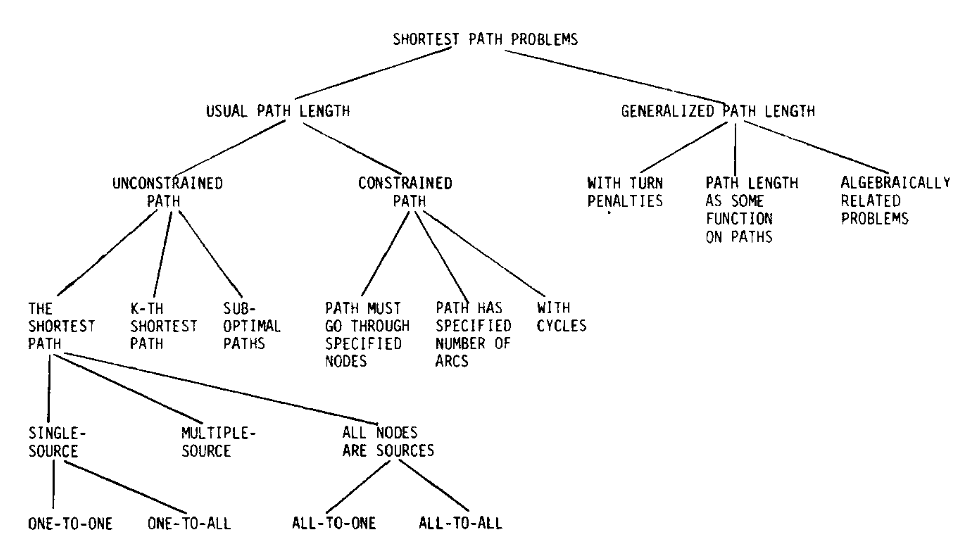
\includegraphics[width=\linewidth]{bilder/shortest path variants tree (Shortest-path algorithms Taxonomy and annotation).png}
	\caption{This image shows a conceptual tree of different variations of shortest path algorithms, taken from \cite{deo_shortest-path_1984}}
	\label{fig:shortestPathTaxonomy}	
\end{figure}

Since the shortest path problem has been well-studied and still continues to advance in terms of the quality of the returned paths as well as in optimizing the running time of algorithms, the number of approaches to solve it is enormous.
The above tree offers a systematic approach to classify problems and most fall into one of two categories: they are either single-source shortest paths (SSSP, on the leftmost branch the two bottom left items) or all-pairs shortest paths(APSP, on the leftmost branch the two bottom right items) \cite{madkour_survey_2017}.
The first  - SSSP - only uses one single starting point and tries to find the one shortest path between it and one or all other vertices.
The second aims to find shortest paths between all vertices of a graph - starting from a specified vertex or from every vertex to every other, which can be necessary for transportation networks and similar use cases. 
Aside from these two categories, many more can be found to describe and sort types of approaches. 
Madkour et al propose a different taxonomy than Deo and Pang did (see \cite{deo_shortest-path_1984} and figure \ref{fig:shortestPathTaxonomy}) to help classify the different algorithms into specific categories. \cite{madkour_survey_2017} 

Which of these algorithms performs best is typically dependent on the type of graph it is being used on, the graph's structure and the specific problem to be solved. 
A graph can be categorized as planar or not, directed or undirected, weighted or not, and carry only non-negative weights or allow negative ones as well, they can contain cycles or be acyclic and many more. 
These different types determine which algorithms can be used as well as which will return better results.
Some algorithms like Dijkstra can - without modifications - only be used on a specific type of graph. 
In this case, the graph needs to have only non negative edges.
Others are modified versions, created specifically to fix problems like graphs with negative edges. 

\subsection{Single Source Shortest Paths}
Following the classification graph (see \ref{fig:shortestPathTaxonomy}), on the bottom left, there is a class \glqq single-source\grqq, which envelops one to one and one to all paths.
This class describes all problems that have a single source node and - following the respective parent nodes - have a usual path length, are unconstrained and find a singular short path that is not an approximation.
These kinds of problems have common use cases in many daily routing problems. 
One to one paths are already described in this chapter's introduction - finding shortest paths to a specified destination \cite{sanders_shortest_2019}.
One to all paths can be useful for cases like fire departments or the police that might need a map of quickest routes for every place in their jurisdiction \cite{sanders_shortest_2019}.

For these, many algorithms have been developed over time, trying to solve more types of problems. 
Some algorithms are for undirected graphs (for example Dijkstra \cite{wayahdi_greedy_2021}), some for directed graphs with non-negative weights or with arbitrary weights but without negative cycles (like Bellman-Ford-Moore \cite{cherkassky_shortest_1996}).
The respective lists are long and for many more specific cases, there are even more specific algorithms \cite{deo_shortest-path_1984, madkour_survey_2017}. 



\subsection{All Pairs Shortest Paths}
The path on the left of the classification graph also shows the class \glqq all nodes are sources\grqq, which encompasses the all to one and all to all cases. 
In these lie all problems where it is necessary to build paths from every node to either a single destination or to all other nodes.
As with single source shortest paths, this branch also describes paths that have a usual length, are unconstrained and give the respective best shortest path for every pair of nodes. 
All to one path calculations can be useful in scenarios where an accident happens and out of all available emergency vehicles, the ones with the shortest paths have to be determined \cite{khamayseh_efficient_2015}.
For all to all paths, many traffic-load calculation problems come to mind. 
For example cases where trains have to be distributed along the rail network \cite{curtis_rewire_2012}.


\subsection{Heuristic Approaches}

Additionally to exact approaches, heuristics can be used to improve the runtime of an algorithm.
A heuristic is a technique that is based on experience or statistical insights.
The downside of using such an approach is, that there will no longer be a guarantee that the result is the global optimum, as heuristics specifically only find partial or approximate solutions to a given problem. 
In many cases where it would take too much time or space to find the actual optimal solution, heuristics can be used to find the best possible solution within the given bounds.

For these, several different ideas have been formed. 
These can then be categorized into construction heuristics, improvement heuristics and meta-heuristics \cite{ropke_heuristic_2005}.
Sometimes, a fourth category for two-phase heuristics is included as well (see \cite{}).

\#TODO is this correct for heuristics in general? The paper refers to heuristics for VRP

Construction heuristics build their solution from a starting point until a certain boundary is reached. 
They typically don't have a separate improvement phase.
Improvement heuristics try to improve an already existing solution.
They perform improvement steps several times until a specified boundary is reached.
These boundaries can be e.g. a time limit or reaching the threshold for a good enough approximation.
(Iterative) Local Search and Neighborhoods are examples of improvement heuristics that can be used to reach a more optimized solution. \cite{laporte_5_2002, ropke_heuristic_2005}



\section{Meta-heuristics}
\label{sec:metaHeuristics}

Meta-heuristics are a form of heuristic approaches.
As such, they also try to find an approximate solution to a problem that is as optimal as possible.
The distinction between classical heuristics and meta-heuristics is, that the latter are combined with additional strategies.
These are used to enable the meta-heuristics to not produce only solution that are locally optimal, but to broaden the search space they can use for finding optima.

Classical heuristics oftentimes carry the inherent risk of only finding a local optimum that can be far from the actual global one.
To reduce this risk, higher level approaches are necessary.
These can include using several neighborhood structures to broaden the search space or entirely new concepts like the Ant Colony approach or Genetic Algorithms. \cite{gendreau_handbook_2010}

The meta-heuristic ideas that will be used in this thesis will be explained in the following subsections.



\subsection{Ant Colony}
\label{subsec:antColonyBackground}

Ant Colony is a meta-heuristic approach that is based on biological ants, ant colonies and how they search food.
Real ants start off by walking around on random paths starting from their nest. 
When they discover a food source, they pick up the food and walk back to their nest.
On this way, they distribute a substance called pheromones.
These can then be detected by other ants and indicate to them, that a path leads to a potentially good food source. 
Other ants then are more likely to follow a path with more pheromone placed on it and will in turn lay down their pheromone as well, leading to an accumulation of these on good paths.
Over time, the pheromones dissipate and when they aren't renewed, will evaporate completely, decreasing the attractiveness of the corresponding path \cite{gendreau_handbook_2010, dorigo_ant_1996}. 

Furthermore, pheromone distribution also inherently leads to using shorter paths. 
When several ants have to choose between paths, they will first select at random.
However, as soon as one ant discovers the food, turns around and distributes its pheromone on the way back, it increases the likelihood of it's path being taken.
Here, the shorter paths will be first to receive more pheromones as the ants returning will be quicker.
Due to the faster accumulation, more ants will choose this shorter path and thus place even more pheromone on it, leading to a self-reinforcing loop that converges when all ants choose the best path only.
Then, all worse paths will loose all their pheromone over time and leave the best result as the only remaining path \cite{gendreau_handbook_2010, dorigo_ant_1996}.

To illustrate pheromone distribution, an example illustrates in figure \ref{fig:antSystemExampleIllustration} how real ants find food and establish the best path towards the source. 
In part \textbf{a} on the left side, there are many ants that run between two points A and E. 
These could be the nest and an interesting food source.
In part \textbf{b} in the middle, an obstacle has been added.
This now leaves the ants with a choice, which path to follow. 
In the beginning, the likelihood of picking either path will be around 50\%.
While taking the path, the ants distribute pheromones on it. 
On the shorter route, the ants will end up reaching the food source earlier, thus returning quicker than the ones who took the long path and distribute more pheromone on the shorter path.
For the first few ants, there will be almost no change in the attractiveness of either path.
However, the more ants take the short tour and return quicker, the more pheromone will accumulate on that path.
This leads to a shift in the attractiveness, making the shorter path more likely to be chosen by later ants.
These ants will in turn again increase the amount of pheromones placed, making the path even more attractive.
So, the ants create a self-reinforcing loop of positive feedback through their pheromones which eventually leads to a state where all ants always choose the shorter option.


\begin{figure}[H]
	\begin{centering}
		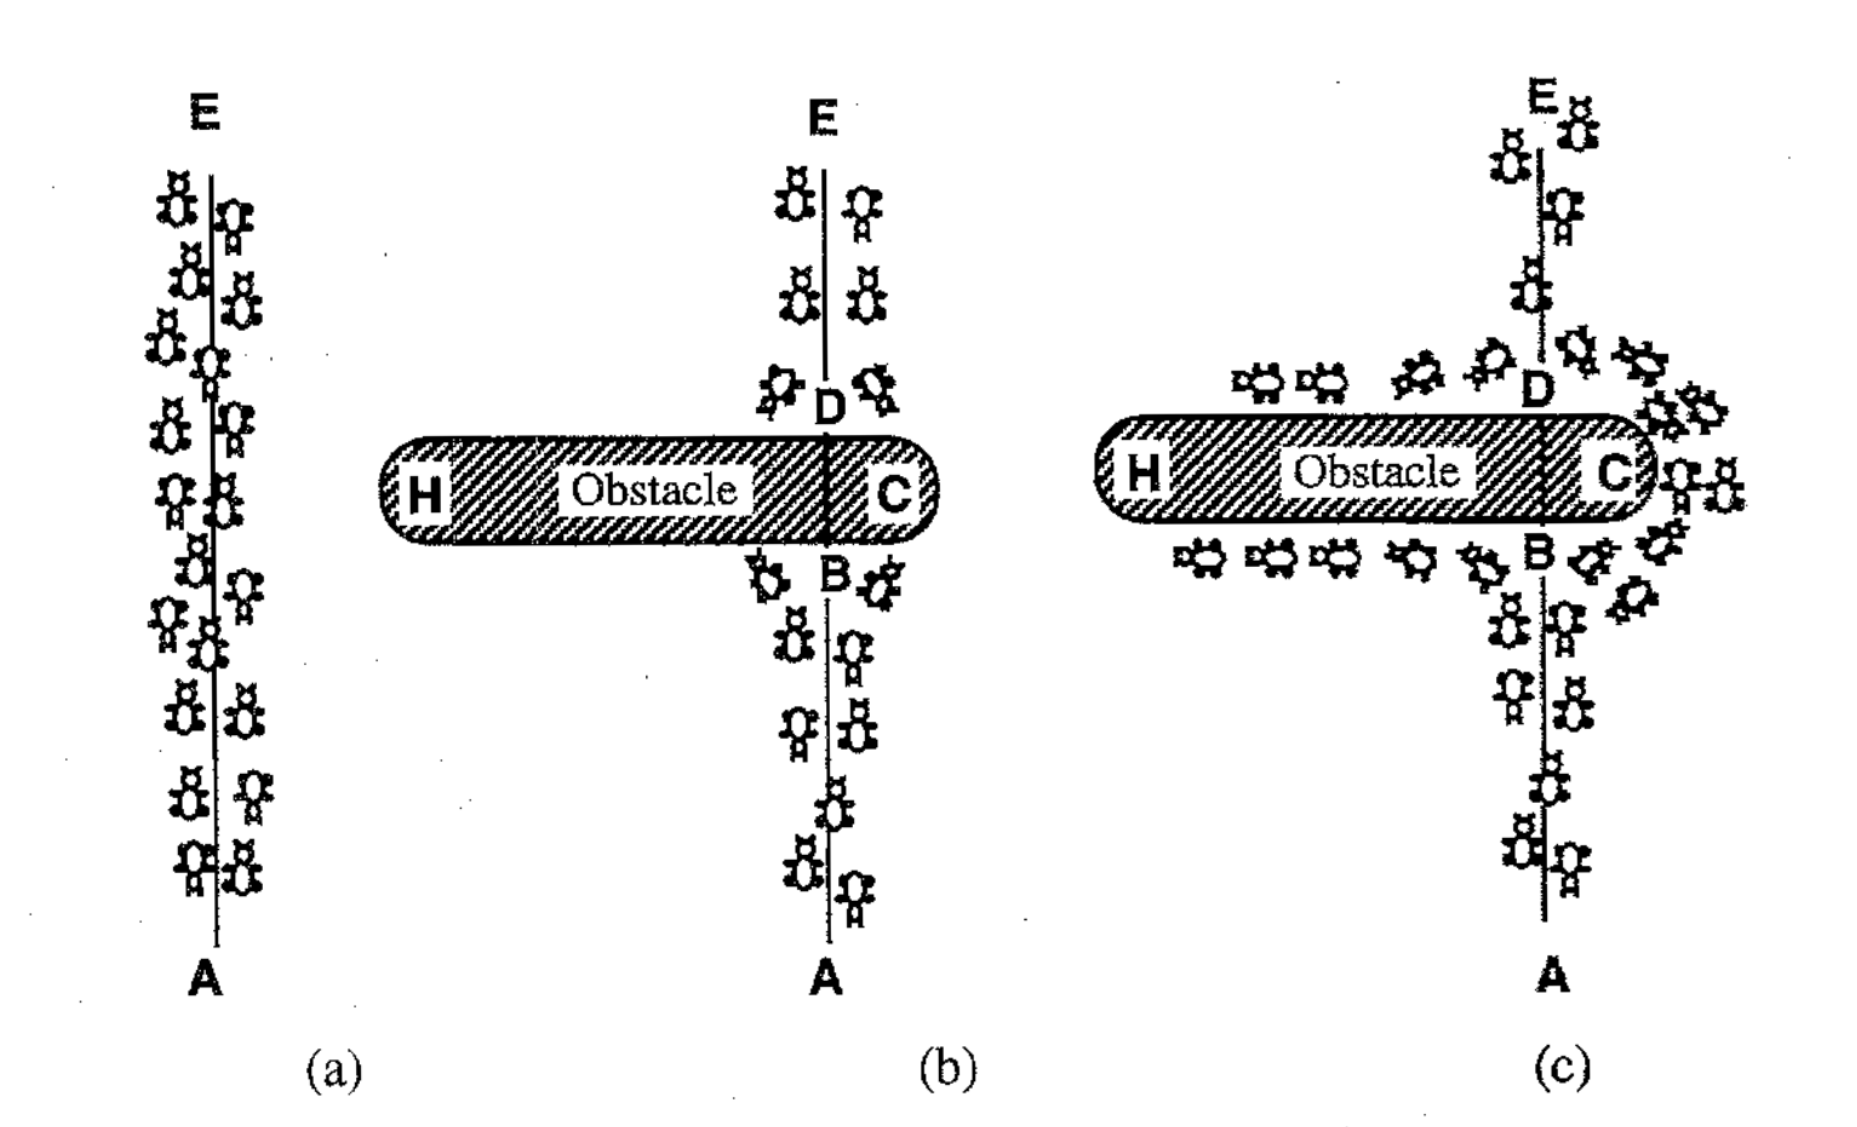
\includegraphics[width=0.8\textwidth]{bilder/antSystemExampleIllustration.png}
		\caption{This figure shows an example of pheromone distribution with real ants. Taken from \textit{Ant System: An Optimization by a Colony of Cooperating Ants}\cite{dorigo_ant_1996}}
		\label{fig:antSystemExampleIllustration}
	\end{centering}
\end{figure}


This behavior can be replicated in virtual graphs for various routing problems.
Ant system has been first introduced in 1990 by Dorigo et al\cite{dorigo_ant_1996}.
In the paper, the authors describe how to use ants for solving the traveling salesman problem (TSP).
This is different from the question of finding a roundtrip with a certain length (plus additional user preferences).
However, in the paper, they stress the adaptability of ant system approaches, showing both versatility and robustness on different example problems\cite{dorigo_ant_1996}.


\subsubsection{Calculations}

To transform the analogy of real ants into an algorithm, some formulas and calculations are needed.
Ants are very simple agents. 
They can only do two things:
Pick the next node to move to and place pheromone on a path.
They communicate with other ant agents through the pheromone trails, making it a decentralized way of communication without the need for a central agent.
For the algorithm, a set amount of $m$ ants moves through the graph, tries to find a good tour and places pheromones on edges.
Every ant has a defined amount of pheromone to place. 
How much of it will be laid on a path can be calculated in several different ways. 
Dorigo et al propose the following three ideas\cite{dorigo_ant_1996}:

\begin{equation}\label{eq:antCycle}
	\Delta\tau_{ij}^k = \begin{cases}
			\frac{Q}{L_k} &\text{if (i,j) $\in$ tour described by $tabu_k(1)$} \\
			0 &\text{otherwise}
	\end{cases}	
\end{equation}


\begin{equation}\label{eq:antDensity}
	\Delta\tau_{ij}^k = \begin{cases}
	Q &\text{if the kth ant goes from i to j between time} \\
	&\text{t to t+1} \\
	0 &\text{otherwise}
\end{cases}	
\end{equation}


\begin{equation}\label{eq:antQuantity}
	\Delta\tau_{ij}^k = \begin{cases}
	\frac{Q}{d_{ij}} &\text{if the kth ant goes from i to j between time} \\
		&\text{to t+1} \\\
	0 &\text{otherwise}
\end{cases}	
\end{equation}

Here, equation \ref{eq:antCycle} is the default the authors used for solving the TSP.
Q is a constant that has to be picked according to the problem in question.
$L_k$ describes the length of the whole tour.
This property makes sense for the TSP setting, but is relatively useless for the case of tours with a fixed length, as it will be the same value for every ant and every run made.
In this case, where the user defines the length of the tour, $L_k$ will only scale the values picked for Q\cite{dorigo_ant_1996}.

Equation \ref{eq:antDensity} only uses the constant Q to describe pheromone placement. 
Here, neither the full tour length nor individual edge costs are taken into account. 
Pheromone is placed evenly on all edges.
This equates to a not-scaled version of equation \ref{eq:antCycle} with the given use-case of a set length for the tour\cite{dorigo_ant_1996}.

The last equation \ref{eq:antQuantity} divides the constant by the length - or the cost - of each edge when it is used. 
Doing this reduces the amount of pheromone placed on longer edges proportionally to shorter edges. 
While this equation is not influenced directly by the fixed length, this property can still cause the equation to be less useful for tours with a specified length than for TSP.
Since tours that are meant to cover a fixed distance are different from the TSP, where a shortest path that visits all selected cities is to be found, the last equation seems like the least promising candidate for useful pheromone distribution\cite{dorigo_ant_1996}.

It is possible to define other ways to calculate the pheromone placement. 
Which option turns out to be the best fitting one will be described in the evaluation chapter \ref{chapter:evaluation}.


Using a suitable formula to calculate the pheromone distribution, this value can then be used to calculate the overall distributed pheromone for each edge $(i,j)$ that was placed by all ants during one iteration.
This value is described by $\Delta\tau_{ij}$ as follows\cite{dorigo_ant_1996}:

\begin{equation}\label{eq:deltaTau}
	\Delta\tau_{ij} = \sum_{k=1}^{m} \Delta\tau_{ij}^k 
\end{equation}

This overall value can then be used to calculate the so called \glqq intensity\grqq{} of the placed pheromone trail.
Since pheromones evaporate over time, this property has to be modeled as well. 
To do this, a new parameter $\rho$ needs to be introduced. It describes how much of the pheromone stays on the trail between two time steps.
So, the overall pheromone intensity can be described by


\begin{equation}\label{eq:trailIntensity}
	\tau_{ij}(t+n) = \rho \cdot \tau_{ij}(t)+\Delta\tau_{ij}^k 
\end{equation}

where $\tau_{ij}(t)$ is the previous pheromone intensity and t+n describes the next time step after one full tour was created in n steps\cite{dorigo_ant_1996}.

Using these calculations, the pheromone intensity on all paths can be represented. 
What's left is determining the probability with which ants will choose a certain edge over the other options.
To do this, two more properties are needed: the visibility of an edge and a tabu-list (or rather a list of allowed nodes).
The tabu-list contains all nodes that have been visited before.
Since roundtrips should - per default - be round rather than the same path run in two directions, this property is needed to ensure no city is visited more than once.
In chapter \ref{chapter:evaluation}, different configurations are tested to represent different shapes and allow for more options users can define. 
Thus, for other shapes, this list is not needed.
The visibility $\nu_{ij}^k$ is calculated using the length of the edge $d_{ij}$ as follows:

\begin{equation}\label{eq:visibility}
	\nu_{ij}^k = \frac{1}{d_{ij}}
\end{equation}

And the transition probability is given by

\begin{equation}\label{eq:transitionProbability}
	p_{ij}^k = \begin{cases}
		\frac{[\tau_{ij}(t)]^{\alpha} \cdot [\nu_{ij}]^{\beta}}{\sum_{k \in allowed_k} [\tau_{ij}(t)]^{\alpha} \cdot [\nu_{ij}]^{\beta}} &\text{if $j \in allowed_k$ }\\
		0 &\text{otherwise}
	\end{cases}
\end{equation}

using all previously defined values to calculate visibility $\nu_{ij}^k$, trail intensity $\tau_{ij}$, pheromone distribution $\Delta\tau_{ij}$ and $\Delta\tau_{ij}^k$.
Here, $\alpha$ and $\beta$ are parameters that influence the weight of visibility and trail intensity.
Higher values of $\alpha$ increase the significance of the pheromones on the trail (setting $\alpha$ to 0 would lead to completely ignoring the pheromone placed) and higher values of $\beta$ increase the importance of the visibility of an edge (making longer edges less attractive as a result)\cite{dorigo_ant_1996}.
These parameters will be experimented with and their influence will be evaluated in chapter \ref{chapter:evaluation}.

In their paper, Dorigo et al suggest middling values for $\alpha$ and $\beta$ in a range of $[0.5,5]$.
They furthermore stated that the best tour was achieved using $\rho = 0.5$ and $Q=100$.
Overall, the results of experimenting with different parameter configurations showed that for very high or very low values of $\alpha$, no good results could be generated \cite{dorigo_ant_1996}.



\# TODO add fomulas and desription how they help constructing paths
\# TODO add how to use for my work

\subsection{Genetic Algorithms}
\label{subsec:geneticAlgorithmsBackground}

\subsection{Simulated Annealing}
\label{subsec:simulatedAnnealingBackground}